\documentclass[hyphens,aspectratio=169]{beamer}
\usepackage{tikz}
\usetikzlibrary{arrows.meta, positioning}
\usepackage{graphicx}
\usepackage{amssymb}
\usepackage{amsmath}
\usepackage{mathtools}
\usepackage{textcomp}
\usepackage{moresize}
\usepackage{framed}
\usepackage{minted}
\usepackage{relsize}
\graphicspath{{../}}
\usetheme{Berlin}
\usecolortheme[RGB={0,95,47}]{structure}
\beamertemplatenavigationsymbolsempty

\makeatletter
\AtBeginEnvironment{minted}{\dontdofcolorbox}
\def\dontdofcolorbox{\renewcommand\fcolorbox[4][]{##4}}
\setbeamertemplate{footline}{}            % removes the entire bottom bar
\makeatother
\title{Action This Day!}
\subtitle{The Mathematics and Machinations that Bested the German Enigma}
\author{Jonah Weinbaum}
\date{
July 28, 2025
}
\begin{document}

\frame{\titlepage}

\section{Action This Day}

\begin{frame}[fragile]{D-Day}
	\begin{center}
		\begin{figure}
			\includegraphics[scale=0.11]{paper/images/dday.jpg}
			\small
			\caption{\emph{Into the Jaws of Death} -- Robert F. Sargent -- June 6, 1944 (D-Day)}
		\end{figure}

	\end{center}
\end{frame}

\begin{frame}[fragile]{D-Day}
	\begin{center}
		\begin{figure}
			\includegraphics[scale=0.3]{paper/images/dummy_tank.jpg}
			\small
			\caption{Inflatable M4 Sherman Tank -- Operation Bodyguard}
		\end{figure}

	\end{center}
\end{frame}

\begin{frame}[fragile]{D-Day}
	Allied forces needed to time the invasion around
	\begin{itemize}
		\item Time of day
		      \pause
		\item Weather
		      \pause
		\item Tides
		      \pause
		\item Phase of the moon
	\end{itemize}

\end{frame}

\begin{frame}[fragile]{D-Day}
	The invasion was scheduled for June 5th,
	\pause
	then postponed to June 6th
	\pause
	\\\\Further postponement would move the plan a month.
\end{frame}

\begin{frame}[fragile]{D-Day}
	\begin{center}
		\begin{figure}
			\includegraphics[scale=0.21]{paper/images/general_eisenhower.jpg}
			\small
			\caption{General Eisenhower's advance command post near Southwick House}
		\end{figure}

	\end{center}
\end{frame}

\begin{frame}[fragile]{D-Day}
	\begin{center}
		\begin{figure}
			\includegraphics[scale=0.105]{paper/images/bletchley_decrypt.jpg}
			\small
			\caption{Example Bletchley Park decrypt}
		\end{figure}

	\end{center}
\end{frame}

\begin{frame}[fragile]{Letter to Winston Churchill}
\end{frame}

\begin{frame}[fragile]{Acknowledgments}
\end{frame}

\begin{frame}[fragile]{Aims of the Thesis}
	\begin{enumerate}
		\item Present a chronological compendium of cryptographic attacks on Enigma -- focused on mathematically inclined readers
		      \pause
		      \vspace{5mm}
		\item Contribute code for analyzing attacks on Enigma
		      \pause
		      \vspace{5mm}

		\item Analyze the Bombe through the lens of modern mathematics and simulation
	\end{enumerate}
\end{frame}

\begin{frame}[fragile]{Aims of the Thesis}
	\begin{enumerate}
		\item Present a chronological compendium of cryptographic attacks on Enigma -- focused on mathematically inclined readers
		      \vspace{5mm}
		\item Contribute code for analyzing attacks on Enigma
		      \vspace{5mm}

		\item {\bf{Analyze the Bombe through the lens of modern mathematics and simulation}}
	\end{enumerate}
\end{frame}

\begin{frame}[fragile]{Thesis Overview}
	\begin{itemize}
		\item Chapter \texttt{I} (The Enigma)
		      \begin{itemize}
			      \item Key space
			      \item Enigma as a permutation
		      \end{itemize}
	\end{itemize}

\end{frame}

\begin{frame}[fragile]{Thesis Overview}
	\begin{itemize}
		\item Chapter \texttt{II} (The Polish Bomba)
		      \begin{itemize}
			      \item Recovering Enigma wirings
			      \item The Grill Method
			      \item The Clock Method
			      \item The Cyclometer
			      \item Bomba Kryptologiczna
			      \item Zygalksi sheets
		      \end{itemize}
	\end{itemize}

\end{frame}


\begin{frame}[fragile]{Thesis Overview}
	\begin{itemize}
		\item Chapter \texttt{III} (The Turing-Welchman Bombe)
		      \begin{itemize}
			      \item The Bombe
			      \item Diagonal board
			      \item Machine gun
			      \item Consecutive stecker knock out
			      \item Banburismus
		      \end{itemize}
	\end{itemize}

\end{frame}

\begin{frame}[fragile]{Thesis Overview}
	\begin{itemize}
		\item Chapter \texttt{IV} (Stops)
		      \begin{itemize}
			      \item Turing's model
			      \item A new cycle type model
			      \item H-M factor
		      \end{itemize}
	\end{itemize}

\end{frame}

\begin{frame}[fragile]{Presentation Overview}
	\begin{enumerate}
		\item The Enigma machine
		      \pause
		      \vspace{5mm}
		\item The Turing-Welchman Bombe
		      \pause
		      \vspace{5mm}

		\item Analysis of the Bombe
	\end{enumerate}

\end{frame}


\part{}

\section{The Enigma}

\begin{frame}[fragile]{}
	\Huge
	\begin{center}
		The Enigma
	\end{center}
\end{frame}

\begin{frame}[fragile]{Overview}
	\begin{center}
		\scalebox{1}{
			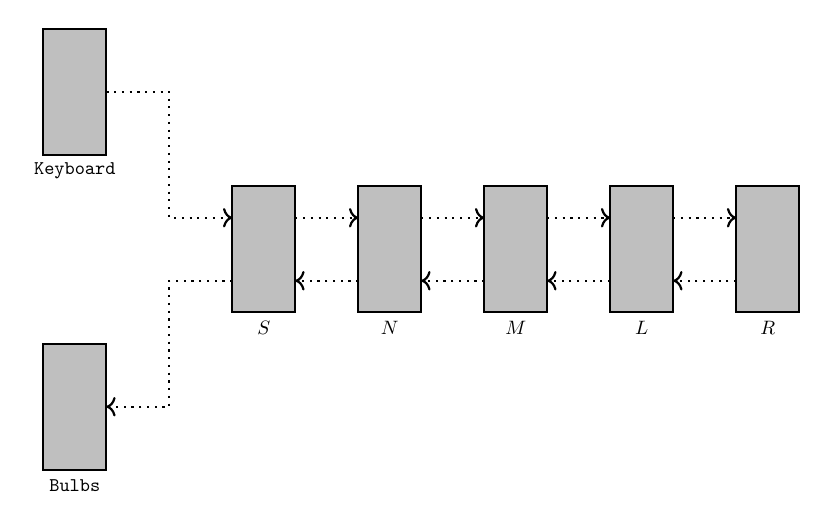
\begin{tikzpicture}[thick, scale=0.4, every node/.style={scale=0.7}]
				\draw[fill=lightgray] (0+5-14, 0+2+5) rectangle (2+5-14,4+2+5) node[midway] {};
				\node at (0+5+1-14, 0+2-0.5+5) {\texttt{Keyboard}};

				\draw[fill=lightgray] (0+5-14, 0+2-5) rectangle (2+5-14,4+2-5) node[midway] {};
				\node at (0+5+1-14, 0+2-0.5-5) {\texttt{Bulbs}};

				\draw[fill=lightgray] (0+5-8, 0+2) rectangle (2+5-8,4+2) node[midway] {};
				\node at (0+5+1-8, 0+2-0.5) {$S$};

				\draw[fill=lightgray] (0+5, 0+2) rectangle (2+5,4+2) node[midway] {};
				\node at (0+5+1, 0+2-0.5) {$M$};

				\draw[fill=lightgray] (0+5+4, 0+2) rectangle (2+5+4,4+2) node[midway] {};
				\node at (0+5+1+4, 0+2-0.5) {$L$};

				\draw[fill=lightgray] (0+5+8, 0+2) rectangle (2+5+8,4+2) node[midway] {};
				\node at (0+5+1+8, 0+2-0.5) {$R$};

				\draw[fill=lightgray] (0+5-4, 0+2) rectangle (2+5-4,4+2) node[midway] {};
				\node at (0+5+1-4, 0+2-0.5) {$N$};

				\draw[->,dotted] (0+5-14+2, 0+2+5+2) -- (0+5-10, 0+2+5+2)
				-- (0+5-10, 0+2+5-2) -- (0+5-8, 0+2+5-2);

				\draw[->,dotted] (0+5-6, 0+2+5-2) -- (0+5-4, 0+2+5-2);
				\draw[->,dotted] (0+5-2, 0+2+5-2) -- (0+5, 0+2+5-2);
				\draw[->,dotted] (0+5+2, 0+2+5-2) -- (0+5+4, 0+2+5-2);
				\draw[->,dotted] (0+5+6, 0+2+5-2) -- (0+5+8, 0+2+5-2);

				\draw[->,dotted] (0+5+8, 0+2+5-4) -- (0+5+6, 0+2+5-4);
				\draw[->,dotted] (0+5+4, 0+2+5-4) -- (0+5+2, 0+2+5-4);
				\draw[->,dotted] (0+5, 0+2+5-4) -- (0+5-2, 0+2+5-4);
				\draw[->,dotted] (0+5-4, 0+2+5-4) -- (0+5-6, 0+2+5-4);

				\draw[->,dotted]  (0+5-8, 0+2+5-4) -- (0+5-10, 0+2+5-4)
				-- (0+5-10, 0+2+5-8) -- (0+5-14+2, 0+2+5-8) ;


			\end{tikzpicture}
		}
	\end{center}
\end{frame}

\begin{frame}[fragile]{Overview}
	\begin{center}
		\scalebox{1}{
			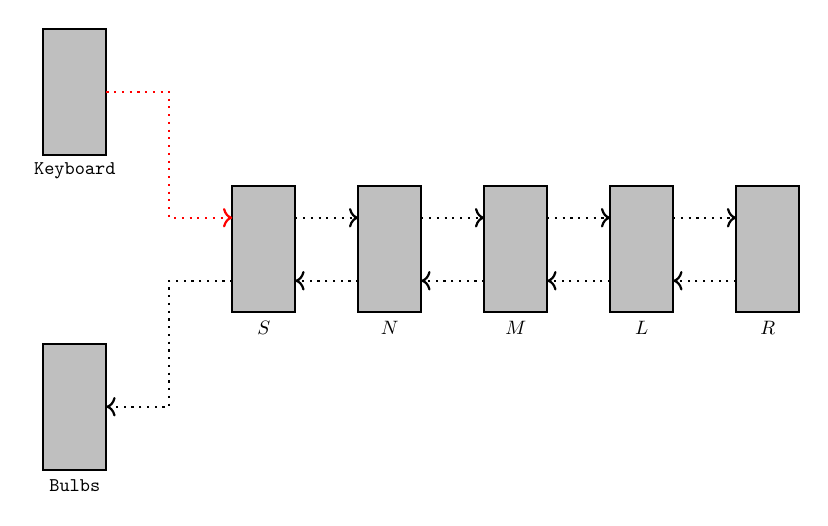
\begin{tikzpicture}[thick, scale=0.4, every node/.style={scale=0.7}]
				\draw[fill=lightgray] (0+5-14, 0+2+5) rectangle (2+5-14,4+2+5) node[midway] {};
				\node at (0+5+1-14, 0+2-0.5+5) {\texttt{Keyboard}};

				\draw[fill=lightgray] (0+5-14, 0+2-5) rectangle (2+5-14,4+2-5) node[midway] {};
				\node at (0+5+1-14, 0+2-0.5-5) {\texttt{Bulbs}};

				\draw[fill=lightgray] (0+5-8, 0+2) rectangle (2+5-8,4+2) node[midway] {};
				\node at (0+5+1-8, 0+2-0.5) {$S$};

				\draw[fill=lightgray] (0+5, 0+2) rectangle (2+5,4+2) node[midway] {};
				\node at (0+5+1, 0+2-0.5) {$M$};

				\draw[fill=lightgray] (0+5+4, 0+2) rectangle (2+5+4,4+2) node[midway] {};
				\node at (0+5+1+4, 0+2-0.5) {$L$};

				\draw[fill=lightgray] (0+5+8, 0+2) rectangle (2+5+8,4+2) node[midway] {};
				\node at (0+5+1+8, 0+2-0.5) {$R$};

				\draw[fill=lightgray] (0+5-4, 0+2) rectangle (2+5-4,4+2) node[midway] {};
				\node at (0+5+1-4, 0+2-0.5) {$N$};

				\draw[->, red ,dotted] (0+5-14+2, 0+2+5+2) -- (0+5-10, 0+2+5+2)
				-- (0+5-10, 0+2+5-2) -- (0+5-8, 0+2+5-2);

				\draw[->,dotted] (0+5-6, 0+2+5-2) -- (0+5-4, 0+2+5-2);
				\draw[->,dotted] (0+5-2, 0+2+5-2) -- (0+5, 0+2+5-2);
				\draw[->,dotted] (0+5+2, 0+2+5-2) -- (0+5+4, 0+2+5-2);
				\draw[->,dotted] (0+5+6, 0+2+5-2) -- (0+5+8, 0+2+5-2);

				\draw[->,dotted] (0+5+8, 0+2+5-4) -- (0+5+6, 0+2+5-4);
				\draw[->,dotted] (0+5+4, 0+2+5-4) -- (0+5+2, 0+2+5-4);
				\draw[->,dotted] (0+5, 0+2+5-4) -- (0+5-2, 0+2+5-4);
				\draw[->,dotted] (0+5-4, 0+2+5-4) -- (0+5-6, 0+2+5-4);

				\draw[->,dotted]  (0+5-8, 0+2+5-4) -- (0+5-10, 0+2+5-4)
				-- (0+5-10, 0+2+5-8) -- (0+5-14+2, 0+2+5-8) ;


			\end{tikzpicture}
		}
	\end{center}
\end{frame}

\begin{frame}[fragile]{The Plugboard}
	\begin{center}
		\includegraphics[]{paper/images/plugboard.jpg}
	\end{center}
\end{frame}

\begin{frame}[fragile]{Overview}
	\begin{center}
		\scalebox{1}{
			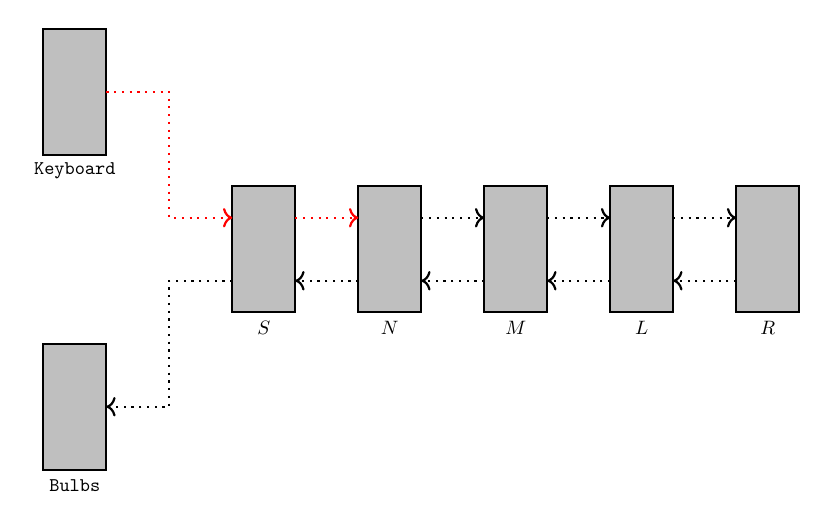
\begin{tikzpicture}[thick, scale=0.4, every node/.style={scale=0.7}]
				\draw[fill=lightgray] (0+5-14, 0+2+5) rectangle (2+5-14,4+2+5) node[midway] {};
				\node at (0+5+1-14, 0+2-0.5+5) {\texttt{Keyboard}};

				\draw[fill=lightgray] (0+5-14, 0+2-5) rectangle (2+5-14,4+2-5) node[midway] {};
				\node at (0+5+1-14, 0+2-0.5-5) {\texttt{Bulbs}};

				\draw[fill=lightgray] (0+5-8, 0+2) rectangle (2+5-8,4+2) node[midway] {};
				\node at (0+5+1-8, 0+2-0.5) {$S$};

				\draw[fill=lightgray] (0+5, 0+2) rectangle (2+5,4+2) node[midway] {};
				\node at (0+5+1, 0+2-0.5) {$M$};

				\draw[fill=lightgray] (0+5+4, 0+2) rectangle (2+5+4,4+2) node[midway] {};
				\node at (0+5+1+4, 0+2-0.5) {$L$};

				\draw[fill=lightgray] (0+5+8, 0+2) rectangle (2+5+8,4+2) node[midway] {};
				\node at (0+5+1+8, 0+2-0.5) {$R$};

				\draw[fill=lightgray] (0+5-4, 0+2) rectangle (2+5-4,4+2) node[midway] {};
				\node at (0+5+1-4, 0+2-0.5) {$N$};

				\draw[->, red,dotted] (0+5-14+2, 0+2+5+2) -- (0+5-10, 0+2+5+2)
				-- (0+5-10, 0+2+5-2) -- (0+5-8, 0+2+5-2);

				\draw[->, red,dotted] (0+5-6, 0+2+5-2) -- (0+5-4, 0+2+5-2);
				\draw[->,dotted] (0+5-2, 0+2+5-2) -- (0+5, 0+2+5-2);
				\draw[->,dotted] (0+5+2, 0+2+5-2) -- (0+5+4, 0+2+5-2);
				\draw[->,dotted] (0+5+6, 0+2+5-2) -- (0+5+8, 0+2+5-2);

				\draw[->,dotted] (0+5+8, 0+2+5-4) -- (0+5+6, 0+2+5-4);
				\draw[->,dotted] (0+5+4, 0+2+5-4) -- (0+5+2, 0+2+5-4);
				\draw[->,dotted] (0+5, 0+2+5-4) -- (0+5-2, 0+2+5-4);
				\draw[->,dotted] (0+5-4, 0+2+5-4) -- (0+5-6, 0+2+5-4);

				\draw[->,dotted]  (0+5-8, 0+2+5-4) -- (0+5-10, 0+2+5-4)
				-- (0+5-10, 0+2+5-8) -- (0+5-14+2, 0+2+5-8) ;


			\end{tikzpicture}
		}
	\end{center}
\end{frame}

\begin{frame}[fragile]{The Rotors}
	\begin{center}
		\scalebox{0.58}{
			\begin{minipage}{0.48\textwidth}
				\centering
				\includegraphics[width=\linewidth]{paper/images/disassembled.png}
			\end{minipage}%
			\hfill
			\begin{minipage}{0.48\textwidth}
				\centering
				\includegraphics[width=0.8\linewidth]{paper/images/entry.jpg}
				\vspace{4mm} % adjust spacing as needed
				\includegraphics[width=0.8\linewidth]{paper/images/exit.jpg}
			\end{minipage}
		}
	\end{center}
\end{frame}

\begin{frame}[fragile]{Overview}
	\begin{center}
		\scalebox{1}{
			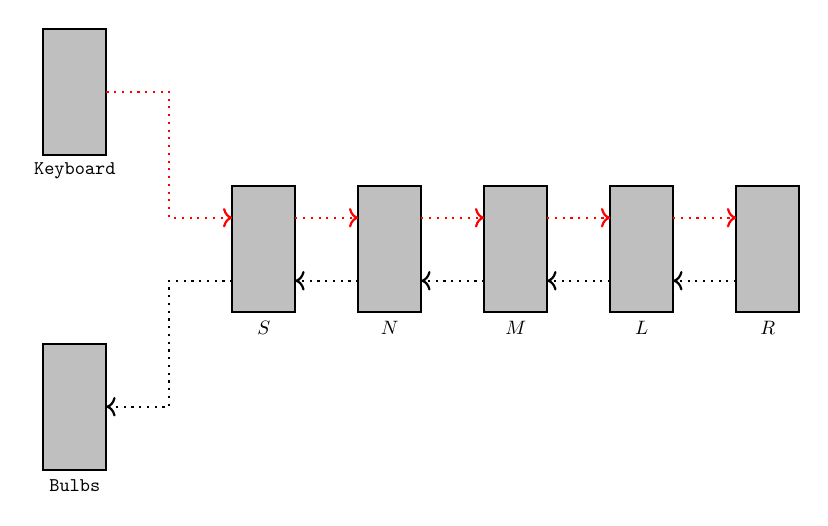
\begin{tikzpicture}[thick, scale=0.4, every node/.style={scale=0.7}]
				\draw[fill=lightgray] (0+5-14, 0+2+5) rectangle (2+5-14,4+2+5) node[midway] {};
				\node at (0+5+1-14, 0+2-0.5+5) {\texttt{Keyboard}};

				\draw[fill=lightgray] (0+5-14, 0+2-5) rectangle (2+5-14,4+2-5) node[midway] {};
				\node at (0+5+1-14, 0+2-0.5-5) {\texttt{Bulbs}};

				\draw[fill=lightgray] (0+5-8, 0+2) rectangle (2+5-8,4+2) node[midway] {};
				\node at (0+5+1-8, 0+2-0.5) {$S$};

				\draw[fill=lightgray] (0+5, 0+2) rectangle (2+5,4+2) node[midway] {};
				\node at (0+5+1, 0+2-0.5) {$M$};

				\draw[fill=lightgray] (0+5+4, 0+2) rectangle (2+5+4,4+2) node[midway] {};
				\node at (0+5+1+4, 0+2-0.5) {$L$};

				\draw[fill=lightgray] (0+5+8, 0+2) rectangle (2+5+8,4+2) node[midway] {};
				\node at (0+5+1+8, 0+2-0.5) {$R$};

				\draw[fill=lightgray] (0+5-4, 0+2) rectangle (2+5-4,4+2) node[midway] {};
				\node at (0+5+1-4, 0+2-0.5) {$N$};

				\draw[->, red,dotted] (0+5-14+2, 0+2+5+2) -- (0+5-10, 0+2+5+2)
				-- (0+5-10, 0+2+5-2) -- (0+5-8, 0+2+5-2);

				\draw[->, red,dotted] (0+5-6, 0+2+5-2) -- (0+5-4, 0+2+5-2);
				\draw[->, red,dotted] (0+5-2, 0+2+5-2) -- (0+5, 0+2+5-2);
				\draw[->, red,dotted] (0+5+2, 0+2+5-2) -- (0+5+4, 0+2+5-2);
				\draw[->, red,dotted] (0+5+6, 0+2+5-2) -- (0+5+8, 0+2+5-2);

				\draw[->,dotted] (0+5+8, 0+2+5-4) -- (0+5+6, 0+2+5-4);
				\draw[->,dotted] (0+5+4, 0+2+5-4) -- (0+5+2, 0+2+5-4);
				\draw[->,dotted] (0+5, 0+2+5-4) -- (0+5-2, 0+2+5-4);
				\draw[->,dotted] (0+5-4, 0+2+5-4) -- (0+5-6, 0+2+5-4);

				\draw[->,dotted]  (0+5-8, 0+2+5-4) -- (0+5-10, 0+2+5-4)
				-- (0+5-10, 0+2+5-8) -- (0+5-14+2, 0+2+5-8) ;


			\end{tikzpicture}
		}
	\end{center}
\end{frame}

\begin{frame}[fragile]{Overview}
	\begin{center}
		\scalebox{1}{
			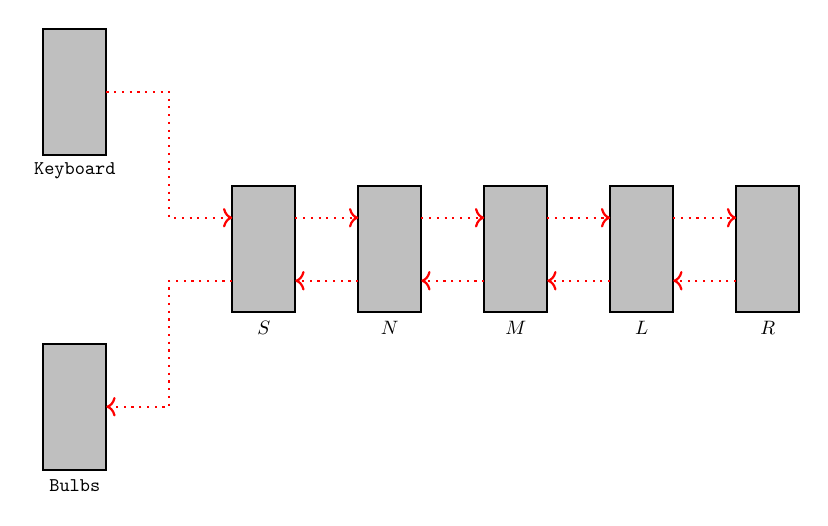
\begin{tikzpicture}[thick, scale=0.4, every node/.style={scale=0.7}]
				\draw[fill=lightgray] (0+5-14, 0+2+5) rectangle (2+5-14,4+2+5) node[midway] {};
				\node at (0+5+1-14, 0+2-0.5+5) {\texttt{Keyboard}};

				\draw[fill=lightgray] (0+5-14, 0+2-5) rectangle (2+5-14,4+2-5) node[midway] {};
				\node at (0+5+1-14, 0+2-0.5-5) {\texttt{Bulbs}};

				\draw[fill=lightgray] (0+5-8, 0+2) rectangle (2+5-8,4+2) node[midway] {};
				\node at (0+5+1-8, 0+2-0.5) {$S$};

				\draw[fill=lightgray] (0+5, 0+2) rectangle (2+5,4+2) node[midway] {};
				\node at (0+5+1, 0+2-0.5) {$M$};

				\draw[fill=lightgray] (0+5+4, 0+2) rectangle (2+5+4,4+2) node[midway] {};
				\node at (0+5+1+4, 0+2-0.5) {$L$};

				\draw[fill=lightgray] (0+5+8, 0+2) rectangle (2+5+8,4+2) node[midway] {};
				\node at (0+5+1+8, 0+2-0.5) {$R$};

				\draw[fill=lightgray] (0+5-4, 0+2) rectangle (2+5-4,4+2) node[midway] {};
				\node at (0+5+1-4, 0+2-0.5) {$N$};

				\draw[->, red,dotted] (0+5-14+2, 0+2+5+2) -- (0+5-10, 0+2+5+2)
				-- (0+5-10, 0+2+5-2) -- (0+5-8, 0+2+5-2);

				\draw[->, red,dotted] (0+5-6, 0+2+5-2) -- (0+5-4, 0+2+5-2);
				\draw[->, red,dotted] (0+5-2, 0+2+5-2) -- (0+5, 0+2+5-2);
				\draw[->, red,dotted] (0+5+2, 0+2+5-2) -- (0+5+4, 0+2+5-2);
				\draw[->, red,dotted] (0+5+6, 0+2+5-2) -- (0+5+8, 0+2+5-2);

				\draw[->, red,dotted] (0+5+8, 0+2+5-4) -- (0+5+6, 0+2+5-4);
				\draw[->, red,dotted] (0+5+4, 0+2+5-4) -- (0+5+2, 0+2+5-4);
				\draw[->, red,dotted] (0+5, 0+2+5-4) -- (0+5-2, 0+2+5-4);
				\draw[->, red,dotted] (0+5-4, 0+2+5-4) -- (0+5-6, 0+2+5-4);

				\draw[->, red,dotted]  (0+5-8, 0+2+5-4) -- (0+5-10, 0+2+5-4)
				-- (0+5-10, 0+2+5-8) -- (0+5-14+2, 0+2+5-8) ;


			\end{tikzpicture}
		}
	\end{center}
\end{frame}

\subsection{Key Space}

\begin{frame}[fragile]{Slide}
\end{frame}

\part{}

\section{Group Theory and Permutations}

\begin{frame}[fragile]{Slide}
\end{frame}

\subsection{Enigma as a Permutation}

\begin{frame}[fragile]{Slide}
\end{frame}

\part{}
\section{The Cyclometer}

\subsection{Characteristics}
\begin{frame}[fragile]{Slide}
\end{frame}

\subsection{The Cyclometer}
\begin{frame}[fragile]{Slide}
\end{frame}

\part{}
\section{The Turing-Welchman Bombe}

\begin{frame}[fragile]{Slide}
\end{frame}

\part{}
\section{Extensions to The Bombe}

\begin{frame}[fragile]{Slide}
\end{frame}

\part{}
\section{Stops}

\begin{frame}[fragile]{Slide}
\end{frame}

\part{}
\section{The H-M Factor}

\subsection{Prior Work}

\begin{frame}[fragile]{Slide}
\end{frame}

\subsection{A New H-M Factor}

\begin{frame}[fragile]{Slide}
\end{frame}

\part{}
\section{Code Contributions}

\begin{frame}[fragile]{Slide}
\end{frame}

\part{}
\section{Future Work}

\begin{frame}[fragile]{Slide}
\end{frame}

\end{document}
